%=======================================================================
\section{Introduction}
\label{sec:intro}

Latent heat thermal energy storage couples a heat transfer fluid to a
phase-change material (PCM) through a wall, and the engineering problem is
almost always the same: the PCM conducts poorly, so the exchanger is finned,
staged, or otherwise elaborated until the phase change can be driven at the
required rate. Designing such an exchanger requires a model that couples a
\emph{heat transfer network} --- convection, wall, fins, and a growing melt
layer --- to a \emph{moving phase boundary}, over a duty cycle, at a cost low
enough to permit parametric study.

Two families of reduced-order model are in common use. Closed-form Stefan
solutions give the front position directly from a prescribed surface
temperature, and are attractive because they are explicit. Energy-balance
formulations instead advance the front from the heat that the network actually
delivers, which enforces conservation between the two sides of the wall. This
paper is concerned with a defect shared by both, and with what has to change to
remove it.

\subsection{The state variable, and what it cannot say}

Both families carry the melt front as a geometric quantity: a layer thickness
$\delta$, or equivalently a melted cross-sectional area $\Amelt$. Ask such a
model for the temperature of the PCM in a given control volume and the only
answer available is the melting temperature $\Tm$, because that is all the state
encodes. While solid remains, the answer is correct, which is why the limitation
is easy to miss.

It stops being correct the moment a control volume completes its phase change.
The network still reports a positive heat flow --- the fluid is still hotter
than $\Tm$, and nothing in the resistance chain knows the PCM is exhausted ---
and the model must do one of two things:

\begin{enumerate}[leftmargin=1.8em,itemsep=2pt]
\item \textbf{Continue melting.} $\Amelt$ grows past the PCM the control volume
  contains. Latent heat is drawn from material that is not there, and local
  melted fractions exceed unity.
\item \textbf{Clip and discard.} Cap $\Amelt$ at the available inventory and
  throw the surplus away. The melted fraction is then physical, but energy is
  not conserved, and the fluid leaves at a temperature that reflects heat which
  went nowhere.
\end{enumerate}

Neither is acceptable, and no refinement of the marching scheme repairs either,
because the deficiency is in the state: a variable counting melted area has no
slot for liquid above $\Tm$ or solid below it. The remedy adopted here is to
integrate enthalpy and recover the melted area from it --- the classical
enthalpy method \cite{Voller1987,Alexiades1993}, applied not to a discretised
field but to the lumped state of a one-dimensional exchanger segment.

\subsection{Contribution}

This paper makes three contributions, all concerning the formulation and its
numerics rather than the application:

\begin{enumerate}[leftmargin=1.8em,itemsep=3pt]
\item \textbf{A lumped enthalpy state for exchanger segments}
  (\S\ref{sec:formulation}). One scalar per segment encodes subcooled solid,
  two-phase and superheated liquid; the melted fraction is confined to $[0,1]$
  by the constitutive relation rather than by a guard, and no heat is ever
  discarded.
\item \textbf{The correct closing conductance} (\S\ref{sec:closure}). Deriving
  the segment equation from control-volume balances yields
  $K=\md c_{p}(1-e^{-\mathrm{NTU}})/\Delta z$, not $\Ui P_{i}$. The two agree
  only as $\mathrm{NTU}\to0$; the naive form lacks the capacity-rate limit and
  therefore permits unphysical behaviour as the wall conductance improves.
\item \textbf{A branchwise-exact integrator} (\S\ref{sec:integration}).
  Explicit stepping is exact on the latent plateau and inadmissible off it. The
  scheme presented solves each branch in closed form, splits steps at branch
  crossings, is unconditionally stable, and makes energy closure structural.
\end{enumerate}

\noindent
Section~\ref{sec:demo} demonstrates the formulation on a PCM-filled wellbore
heat exchanger and reports the physical consequence that motivated the work: the
self-levelling of the melt distribution.

%=======================================================================
\section{Enthalpy formulation}
\label{sec:formulation}

\subsection{Configuration and hypotheses}

Consider a tube of developed length $L_{\mathrm{tube}}$ carrying a
single-phase fluid at mass flow $\md$, surrounded by PCM. The tube is divided
into $n_{s}$ segments of length $\Delta z$ along the developed coordinate $s$.
Each segment owns a PCM cross-section $\Aav$, and the melting temperature may
vary from segment to segment, permitting an axially graded (cascaded) store in
which $\Tm$ follows the fluid glide.

The following are assumed throughout.

\begin{description}[leftmargin=1.9em,itemsep=2pt]
\item[H1] Quasi-steady conduction in the melt layer: its temperature profile is
  the steady cylindrical profile for the instantaneous front position. The
  hypothesis is controlled by the Stefan number
  $\mathrm{Ste}=c_{p}\Delta T/\hm$.
\item[H2] No axial conduction in the wall or the PCM; segments couple only
  through the fluid stream.
\item[H3] The melt region is a concentric annulus of uniform thickness $\delta$
  about each tube, and fronts about neighbouring tubes do not interact.
\item[H4] Conduction only in the melt; no natural convection in the liquid PCM.
\item[H5] One PCM temperature per segment: the state is lumped, with no radial
  resolution of temperature \emph{within} a phase.
\item[H6] Adiabatic outer boundary.
\item[H7] Incompressible single-phase fluid, treated as quasi-steady.
\end{description}

\subsection{Why enthalpy rather than temperature}

The natural repair for the deficiency of \S\ref{sec:intro} is to carry a PCM
temperature alongside the melted area. It is the wrong repair, for a reason that
recurs throughout phase-change modelling: at a phase change, temperature is not
invertible. During melting the PCM remains at $\Tm$ while its energy content
climbs by the entire latent heat, so $T$ carries no information whatever
throughout the process that dominates the problem. A pair $(T,\Amelt)$ works,
but obliges the code to decide at every step which member is active, keep the
two consistent, and handle the instants at which the active member changes.

Enthalpy is invertible. Every state of the PCM corresponds to exactly one value
of the enthalpy, and the enthalpy increases monotonically as heat is added. A
single scalar per segment therefore encodes all three regimes, and the regime is
read from the value rather than tracked separately
(Fig.~\ref{fig:enthalpy-curve}).

\begin{figure}[htbp]
\centering
\begin{tikzpicture}[>=Stealth, scale=0.95]
  \draw[->,thick] (0,0) -- (9.6,0) node[right] {$\Tpcm$};
  \draw[->,thick] (0,0) -- (0,5.8) node[above] {$E'$};
  \draw[dashed,gray] (4.9,0) -- (4.9,5.4);
  \node[below] at (4.9,0) {$\Tm$};
  \draw[dashed,gray] (0,1.5) -- (4.9,1.5) node[pos=0,left] {$0$};
  \draw[dashed,gray] (0,3.5) -- (4.9,3.5) node[pos=0,left] {$\Elat$};
  \draw[very thick] (1.2,0.05) -- (4.9,1.5);
  \draw[very thick] (4.9,1.5) -- (4.9,3.5);
  \draw[very thick] (4.9,3.5) -- (8.9,5.05);
  \node[align=left,font=\small,anchor=west] at (0.85,2.65)
    {solid, subcooled\\[1pt] slope $C_{s}$};
  \node[align=center,font=\small] at (6.9,5.3)
    {liquid, superheated\\[1pt] slope $C_{l}$};
  \draw[<->,thick,black!60] (4.55,1.5) -- (4.55,3.5);
  \node[font=\small,align=right,anchor=east,black!70] at (4.4,1.95)
    {latent heat\\$\rhom\hm\Aav$};
  \filldraw (4.9,2.6) circle (1.6pt);
  \draw[->,black!60] (5.9,1.75) -- (4.99,2.53);
  \node[font=\small,align=left,anchor=west,black!70] at (5.95,1.6)
    {position here is\\$\Amelt = E'/(\rhom\hm)$};
\end{tikzpicture}
\caption{The constitutive curve, Eq.~\eqref{eq:enth-curve}. Read as $E'(T)$ it
is multivalued at $\Tm$, which is why temperature cannot serve as the state.
Read as $T(E')$ --- the direction used here --- it is single-valued everywhere,
and position along the vertical segment is the melted fraction.}
\label{fig:enthalpy-curve}
\end{figure}

\subsection{State and capacities}

Let $E'$ be the enthalpy per unit tube length of the PCM belonging to one
segment, measured from a datum of fully solid material at $\Tm$. The datum is
arbitrary; this choice places the two branch boundaries at $0$ and $\Elat$,
which shortens every test in the implementation. With
\begin{equation}
  \Elat = \rhom\hm\Aav,
  \qquad
  C_{s} = \rhom c_{p,s}\Aav,
  \qquad
  C_{l} = \rhom c_{p,l}\Aav,
  \label{eq:caps}
\end{equation}
the latent capacity and the two sensible capacities per unit tube length, the
constitutive curve and the melted area are
\begin{equation}
  \Tpcm =
  \begin{dcases}
    \Tm + E'/C_{s}, & E' < 0 \quad\text{(solid, subcooled)},\\[2pt]
    \Tm, & 0 \le E' \le \Elat \quad\text{(two-phase)},\\[2pt]
    \Tm + \bigl(E'-\Elat\bigr)/C_{l},
      & E' > \Elat \quad\text{(liquid, superheated)},
  \end{dcases}
  \label{eq:enth-curve}
\end{equation}
\begin{equation}
  \Amelt = \frac{\min\!\bigl(\max(E',0),\,\Elat\bigr)}{\rhom\hm},
  \qquad
  \varepsilon_{\mathrm{local}} = \frac{\Amelt}{\Aav} \in [0,1].
  \label{eq:amelt}
\end{equation}

The saturation in Eq.~\eqref{eq:amelt} is not a guard added to suppress bad
behaviour; it is the definition. Melted area saturates because a segment cannot
melt PCM it does not own, and superheat is where the additional energy goes.
Consequently $\varepsilon_{\mathrm{local}}\in[0,1]$ is \emph{structural}: no
code path can violate it, and no test for it is required.

\subsection{Recovering the layer thickness}

The resistance network requires $\delta$, not $\Amelt$. For a tube of outer
radius $r_{e}$ carrying $n_{f}$ longitudinal fins of thickness $t_{f}$ and
radial length $L_{f}$, the fin metal occupies part of the annulus and must be
excluded from the melted PCM area:
\begin{equation}
  \Amelt = \pi\left[(r_{e}+\delta)^{2}-r_{e}^{2}\right]
           - n_{f}t_{f}\min\!\left(\delta,L_{f}\right),
  \label{eq:area-fins}
\end{equation}
which inverts in closed form on each branch,
\begin{align}
  \delta \le L_{f}: &\quad
    \pi\delta^{2}+\left(2\pi r_{e}-n_{f}t_{f}\right)\delta-\Amelt = 0,
  \label{eq:delta-in}\\
  \delta > L_{f}: &\quad
    \pi\delta^{2}+2\pi r_{e}\delta-\left(\Amelt+n_{f}t_{f}L_{f}\right) = 0 .
  \label{eq:delta-out}
\end{align}
For $n_{f}=0$ both reduce to
$\delta=\sqrt{r_{e}^{2}+\Amelt/\pi}-r_{e}$.

The melt layer then enters the network as a cylindrical conduction shell,
\begin{equation}
  h_{e} = \frac{\km}{r_{e}\ln\!\left(1+\delta/r_{e}\right)},
  \label{eq:he}
\end{equation}
and the overall coefficient on the inner area, with fin efficiency $\etaf$,
overall surface efficiency $\etao$ and finned perimeter $P_{T}$, is
\begin{equation}
  \Ui = \left[\frac{1}{h_{i}} + R''_{f,i}
        + \frac{r_{i}}{k_{w}}\ln\frac{r_{e}}{r_{i}}
        + \frac{2\pi r_{i}}{P_{T}\,\etao\,h_{e}}\right]^{-1}.
  \label{eq:Ui}
\end{equation}

The single change relative to an area-based formulation is that the outer
boundary of this chain sits at $\Tpcm$, not at $\Tm$. It coincides with $\Tm$
only while solid remains. Section~\ref{sec:demo} shows that this one
substitution is responsible for the principal physical result.

%=======================================================================
\section{The segment equation and its closure}
\label{sec:closure}

Equation~\eqref{eq:ode} below is short enough to look like a definition. It is
not: it follows from energy balances on two control volumes and the elimination
of the quantity they share. The derivation is given in full because the closing
conductance is not the one a reader would write down unaided.

\subsection{Two control volumes}

Fix a segment $j$ spanning $s\in[s_{j},s_{j+1}]$, $\Delta z=s_{j+1}-s_{j}$. Two
control volumes share the tube wall over that interval: \textbf{CV\,1}, the PCM
belonging to the segment --- cross-section $\Aav$, stationary, closed --- and
\textbf{CV\,2}, the fluid within the tube over the same interval, open, entering
at $T_{j}$ and leaving at $T_{j+1}$. Write $q'_{j}$ for the heat per unit tube
length crossing from CV\,2 into CV\,1.

\subsection{The PCM balance}

CV\,1 is closed and stationary, so the first law reduces to a statement about
its enthalpy. With the axial (H2) and outer-boundary (H6) terms dropped,
\begin{equation}
  \boxed{\;\frac{\mathrm{d}E'_{j}}{\mathrm{d}t} = q'_{j}\;}
  \label{eq:pcm-balance}
\end{equation}

\subsection{The fluid balance}

For incompressible single-phase flow without viscous dissipation, the energy
equation per unit tube length is
\begin{equation}
  \rho A_{\mathrm{flow}} c_{p}\frac{\partial T}{\partial t}
  + \md c_{p}\frac{\partial T}{\partial s} = -q'(s).
  \label{eq:fluid-pde}
\end{equation}
Hypothesis H7 drops the first term. The approximation is justified by the
separation between the fluid transit time and the timescale of the PCM state,
and its cost is an unresolved startup transient of one transit at the beginning
of each half-cycle; \S\ref{sec:demo} quantifies both for the case studied.

With CV\,1 presenting a single temperature to the whole segment (H5), the local
flux closes on the network,
\begin{equation}
  q'(s) = \Ui\,(2\pi r_{i})\left[T(s)-\Tpcm\right].
  \label{eq:local-flux}
\end{equation}
The inner perimeter $2\pi r_{i}$ appears rather than $P_{T}$ because $\Ui$ was
referred to the inner area in Eq.~\eqref{eq:Ui}; the finned perimeter is already
inside it. Using $P_{T}$ here would count the fins twice.

\subsection{Integration across the segment}

Substituting Eq.~\eqref{eq:local-flux} into the steady form of
Eq.~\eqref{eq:fluid-pde}, with $\Tpcm$ and $\Ui$ held constant over the segment,
gives a linear ordinary differential equation in $s$ whose solution is the
single-stream heat exchanger result:
\begin{equation}
  T_{j+1} = \Tpcm + \left(T_{j}-\Tpcm\right)e^{-\mathrm{NTU}_{j}},
  \qquad
  \mathrm{NTU}_{j} = \frac{2\pi r_{i}\,\Ui\,\Delta z}{\md\,c_{p}}.
  \label{eq:ntu}
\end{equation}
One stream carries a finite capacity rate $\md c_{p}$; the other is an
isothermal reservoir of infinite capacity rate, with effectiveness
$\varepsilon=1-e^{-\mathrm{NTU}}$. The reservoir idealisation is precisely what
the lumped state of H5 licenses.

\subsection{The closure, and why the conductance is not $\Ui P_{i}$}

The heat the fluid gives up over the segment is the enthalpy it loses, so from
Eq.~\eqref{eq:ntu},
\begin{equation}
  \boxed{\;
  q'_{j} = K_{j}\left(T_{j}-\Tpcm\right),
  \qquad
  K_{j} = \frac{\md c_{p}\left(1-e^{-\mathrm{NTU}_{j}}\right)}{\Delta z}.
  \;}
  \label{eq:K}
\end{equation}
Combining Eqs.~\eqref{eq:pcm-balance}, \eqref{eq:K} and \eqref{eq:enth-curve}
closes the system:
\begin{equation}
  \boxed{\;
  \frac{\mathrm{d}E'}{\mathrm{d}t}
  = K\left(T_{j}-\Tpcm(E')\right)
  \;}
  \label{eq:ode}
\end{equation}
with one unknown per segment; everything else is geometry, a property, or the
upstream fluid temperature handed down by the preceding segment.

The naive closure evaluates Eq.~\eqref{eq:local-flux} at $T(s)\approx T_{j}$,
giving $q'_{j}\approx 2\pi r_{i}\Ui(T_{j}-\Tpcm)$. Comparing,
\begin{equation}
  \frac{K_{j}}{2\pi r_{i}\Ui}
  = \frac{1-e^{-\mathrm{NTU}_{j}}}{\mathrm{NTU}_{j}} \le 1,
  \label{eq:K-ratio}
\end{equation}
and the two limits say what the difference means. As $\mathrm{NTU}\to0$ the
ratio tends to unity: the fluid barely cools across the segment and the naive
closure is correct. As $\mathrm{NTU}\to\infty$, $K\to\md c_{p}/\Delta z$, a
finite limit set by the \emph{fluid} rather than the wall --- a segment cannot
absorb more than the stream delivers to it. The naive closure has no such limit:
it permits $T_{j+1}$ to fall below $\Tpcm$, that is, heat flowing from cold to
hot, at a rate growing without bound as $\Ui$ improves. The discrepancy is
largest where the melt layer is thinnest and the exchanger best, which is where
the model is most active.

\subsection{Closure is structural}

Equation~\eqref{eq:K} is not evaluated independently of
Eq.~\eqref{eq:pcm-balance}. The implementation integrates
Eq.~\eqref{eq:pcm-balance} over the step and \emph{reports}
\begin{equation}
  q'_{j} = \frac{E'^{\,n+1}-E'^{\,n}}{\Delta t},
  \label{eq:qfromE}
\end{equation}
then drops the fluid temperature by exactly that amount,
$T_{j+1}=T_{j}-q'_{j}\Delta z/(\md c_{p})$. Whatever the PCM gained, the fluid
lost, to machine precision, with no possibility of drift. It should be stressed
that this is a \emph{consistency} property and not evidence of correctness: the
two operations are inverse, so a small residual measures floating-point
arithmetic and nothing else.

%=======================================================================
\section{Branchwise-exact time integration}
\label{sec:integration}

\subsection{Why explicit stepping is inadmissible}

Equation~\eqref{eq:ode} is nonlinear, because $\Tpcm(E')$ is piecewise, but
affine within each branch of Eq.~\eqref{eq:enth-curve}. The distinction governs
the choice of integrator.

On the latent plateau $\Tpcm=\Tm$ is constant and does not respond to $E'$ at
all. The segment behaves as though its heat capacity were infinite,
Eq.~\eqref{eq:ode} reduces to $\mathrm{d}E'/\mathrm{d}t=\text{const}$, and an
explicit Euler step is not merely stable but exact. This is the regime an
area-based formulation occupies permanently, which explains why the constraint
derived below has not previously been a concern: explicit stepping was safe for
a structural reason, not a fortunate one.

Introducing sensible capacity makes the capacity finite. Equation~\eqref{eq:ode}
becomes a relaxation equation with time constant $C/K$, and explicit Euler
requires $\Delta t < C/K$. Logarithmic time grids, which are the natural choice
for a diffusion-limited process, violate this at late times by a wide margin;
\S\ref{sec:demo} gives the figures for the case studied, where the final step
exceeds the limit by a factor of $7.7$ and an explicit implementation diverges.

\subsection{The scheme}

Rather than reduce $\Delta t$ --- which for a logarithmic grid multiplies the
cost by some three orders of magnitude --- the linearity within each branch is
exploited and each branch integrated in closed form. Holding $T_{j}$ fixed
across the step,
\begin{equation}
  E'(t+\Delta t) =
  \begin{dcases}
    E' + K\left(T_{j}-\Tm\right)\Delta t,
      & \text{plateau,}\\[4pt]
    \Eeq + \bigl(E'-\Eeq\bigr)e^{-K\Delta t/C},
      & \text{sensible branches,}
  \end{dcases}
  \label{eq:exact}
\end{equation}
with the equilibrium enthalpy and relevant capacity
\begin{equation}
  \left(C,\Eeq\right) =
  \begin{cases}
    \left(C_{s},\;C_{s}\left(T_{j}-\Tm\right)\right), & E'<0,\\[3pt]
    \left(C_{l},\;\Elat+C_{l}\left(T_{j}-\Tm\right)\right), & E'>\Elat.
  \end{cases}
  \label{eq:Eeq}
\end{equation}
$\Eeq$ is the enthalpy at which the PCM would sit in equilibrium with the fluid:
the state the segment relaxes toward and never reaches. The exponential is
unconditionally stable and monotone, so no step, however large, can overshoot
it. That is precisely the property explicit Euler lacks.

\subsection{Branch crossings}

A step may begin in one branch and end in another, in which case it is split at
the crossing. With $E'_{b}$ the boundary being approached ($0$ or $\Elat$), the
crossing time is
\begin{equation}
  t^{*} =
  \begin{dcases}
    \frac{E'_{b}-E'}{K\left(T_{j}-\Tm\right)}, & \text{from the plateau},\\[8pt]
    \frac{C}{K}\ln\!\left(\frac{E'-\Eeq}{E'_{b}-\Eeq}\right),
      & \text{from a sensible branch}.
  \end{dcases}
  \label{eq:crossing}
\end{equation}
If $t^{*}<\Delta t$ the state is advanced to $E'_{b}$, the remaining
$\Delta t-t^{*}$ is integrated in the adjacent branch, and the test repeated.
Only a small number of crossings can occur within one step, so the loop is
bounded.

\begin{table}[htbp]
\centering
\caption{Algorithm: advance one segment over $\Delta t$.}
\label{tab:algorithm}
\begin{tabular}{@{}r l@{}}
\toprule
 & \\[-8pt]
1 & $t_{\mathrm{left}} \leftarrow \Delta t$, \quad $E'_{0}\leftarrow E'$ \\
2 & \textbf{while} $t_{\mathrm{left}}>0$: \\
3 & \quad identify the branch containing $E'$ \\
4 & \quad compute $t^{*}$ from Eq.~\eqref{eq:crossing} toward the branch boundary \\
5 & \quad \textbf{if} $t^{*} \ge t_{\mathrm{left}}$: advance by Eq.~\eqref{eq:exact}
        over $t_{\mathrm{left}}$; \textbf{break} \\
6 & \quad \textbf{else}: set $E'\leftarrow E'_{b}\pm\epsilon$;\quad
        $t_{\mathrm{left}} \leftarrow t_{\mathrm{left}}-t^{*}$ \\
7 & \textbf{return} $E'$, \quad $q' = (E'-E'_{0})/\Delta t$ \\[2pt]
\bottomrule
\end{tabular}
\end{table}

\paragraph{A note on the boundary test.}
Step 6 of Table~\ref{tab:algorithm} displaces the state just past the boundary
by $\epsilon=10^{-9}\max(\Elat,1)$ rather than placing it exactly on the
boundary. This is necessary rather than cosmetic. If the branch test uses closed
intervals, a state landing exactly on $\Elat$ is still classified as two-phase;
the plateau branch then computes $t^{*}=0$, advances the state to where it
already is, subtracts zero from the remaining time, and repeats indefinitely.
The segment is pinned at the boundary and never enters the liquid branch. The
symptom is not a failure but an apparent success --- every segment reporting a
melted fraction of exactly unity and zero superheat. The general point is that
where a solver switches on the sign of a quantity, the side of the boundary to
which equality belongs must be chosen deliberately, and the state must not be
able to come to rest there.

%---------------------------------------------------------------------
\begin{figure}[htbp]
\centering
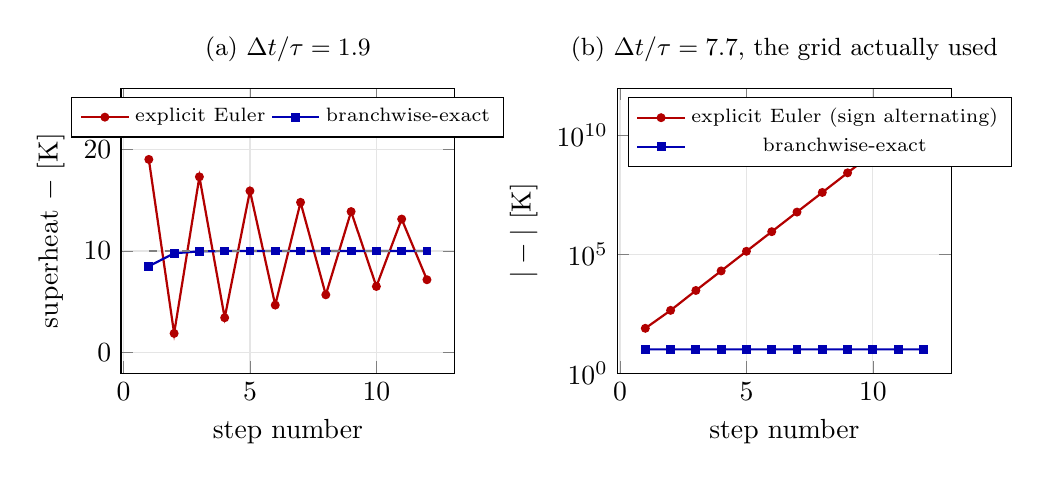
\begin{tikzpicture}
\begin{axis}[width=0.48\linewidth,height=5.2cm,
  xlabel={step number}, ylabel={superheat $\Tpcm-\Tm$ [K]},
  title={\small (a) $\Delta t/\tau=1.9$}, ymin=-2, ymax=26,
  legend style={font=\scriptsize,at={(0.5,0.97)},anchor=north},
  legend columns=2,
  grid=both, grid style={gray!20}]
\addplot[thick,mark=*,mark size=1.2pt,red!70!black] coordinates {(1,19.0) (2,1.9) (3,17.29) (4,3.439) (5,15.9049) (6,4.6856) (7,14.783) (8,5.6953) (9,13.8742) (10,6.5132) (11,13.1381) (12,7.1757)};
\addlegendentry{explicit Euler}
\addplot[thick,mark=square*,mark size=1.2pt,blue!70!black] coordinates {(1,8.5043) (2,9.7763) (3,9.9665) (4,9.995) (5,9.9993) (6,9.9999) (7,10.0) (8,10.0) (9,10.0) (10,10.0) (11,10.0) (12,10.0)};
\addlegendentry{branchwise-exact}
\addplot[dashed,gray,domain=1:12,forget plot] {10};
\end{axis}
\begin{axis}[width=0.48\linewidth,height=5.2cm,at={(0.52\linewidth,0)},
  xlabel={step number}, ylabel={$|\Tpcm-\Tm|$ [K]}, ymode=log,
  title={\small (b) $\Delta t/\tau=7.7$, the grid actually used},
  ymin=1, ymax=1e12, legend style={font=\scriptsize,at={(0.03,0.97)},anchor=north west},
  grid=both, grid style={gray!20}]
\addplot[thick,mark=*,mark size=1.2pt,red!70!black] coordinates {
  (1,77) (2,438.9) (3,3017.6) (4,20141) (5,135023) (6,904574)
  (7,6.0607e6) (8,4.0607e7) (9,2.7207e8) (10,1.8228e9) (11,1.2213e10) (12,8.1827e10)};
\addlegendentry{explicit Euler (sign alternating)}
\addplot[thick,mark=square*,mark size=1.2pt,blue!70!black] coordinates {
  (1,9.9955) (2,10) (3,10) (4,10) (5,10) (6,10) (7,10) (8,10) (9,10) (10,10) (11,10) (12,10)};
\addlegendentry{branchwise-exact}
\end{axis}
\end{tikzpicture}
\caption{Response of a single segment on the liquid branch, driven by fluid
\SI{10}{\kelvin} above $\Tm$ with $\tau=C_{l}/K=\SI{1102}{\second}$.
(a) At $\Delta t/\tau=1.9$ explicit Euler oscillates about the equilibrium
while remaining bounded. (b) At $\Delta t/\tau=7.7$ --- the ratio the
logarithmic grid of Table~\ref{tab:stability} actually reaches at the end of a
charge --- it diverges, alternating in sign and passing
\SI{8e10}{\kelvin} within twelve steps. The branchwise-exact scheme is
monotone and correct at every step size, because Eq.~\eqref{eq:exact} cannot
overshoot $\Eeq$.}
\label{fig:stability}
\end{figure}


%---------------------------------------------------------------------
\begin{figure}[htbp]
\centering
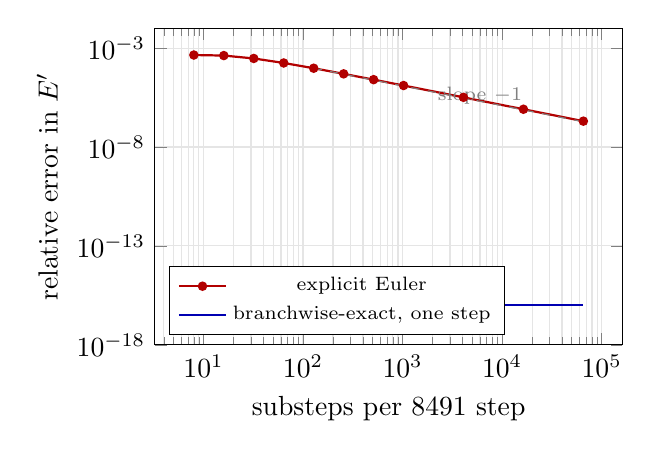
\begin{tikzpicture}
\begin{axis}[width=0.62\linewidth,height=5.6cm,
  xlabel={substeps per \SI{8491}{\second} step}, ylabel={relative error in $E'$},
  xmode=log, ymode=log, ymin=1e-18, ymax=1e-2,
  legend style={font=\scriptsize,at={(0.03,0.03)},anchor=south west},
  grid=both, grid style={gray!20}]
\addplot[thick,mark=*,mark size=1.3pt,red!70!black] coordinates {(8,4.4986e-4) (16,4.2272e-4) (32,3.0168e-4) (64,1.7837e-4) (128,9.6617e-5) (256,5.0229e-5) (512,2.5602e-5) (1024,1.2924e-5) (4096,3.2541e-6) (16384,8.1497e-7) (65536,2.0383e-7)};
\addlegendentry{explicit Euler}
\addplot[thick,blue!70!black,domain=8:65536,samples=2] {1e-16};
\addlegendentry{branchwise-exact, one step}
\addplot[dashed,gray,domain=128:65536,samples=2,forget plot] {1.24e-2/x};
\node[font=\scriptsize,gray] at (axis cs:6000,4e-6) {slope $-1$};
\end{axis}
\end{tikzpicture}
\caption{Error after advancing one segment through a single \SI{8491}{\second}
grid step, against the number of explicit substeps used. Explicit Euler is
first order once it is stable ($\ge 8$ substeps; below that it is not), and
needs of order $10^{4}$ substeps to reach $10^{-6}$. The branchwise-exact
scheme returns the closed-form solution of the branch, so its error is zero to
machine precision in a \emph{single} step --- plotted at $10^{-16}$ for
visibility.}
\label{fig:convergence}
\end{figure}


\subsection{Verification}
\label{sec:verification}

The scheme was verified against a brute-force explicit integration of
Eq.~\eqref{eq:ode} using \num{200000} substeps, over a complete charge and
discharge, including steps crossing branch boundaries. Agreement is
$3\times10^{-13}$ in relative terms, which is machine precision. The two
calculations share no code path beyond Eq.~\eqref{eq:enth-curve}, so this is a
genuine verification of the integrator rather than a consistency check.

Energy closure, by contrast, is structural under Eq.~\eqref{eq:qfromE} and
therefore proves nothing about correctness; it is reported here only to
establish that no drift is present.

